% =============================================================================
% File:  sample_slides.tex --  Example of the use of the Falkor Beamer theme
% Author(s): Sebastien Varrette <Sebastien.Varrette@uni.lu>
% Time-stamp: <Mar 2014-04-29 16:06 svarrette>
%
% Copyright (c) 2012 Sebastien Varrette <Sebastien.Varrette@uni.lu>
% .             http://varrette.gforge.uni.lu
%
% For more information:
% - LaTeX: http://www.latex-project.org/
% - Beamer: https://bitbucket.org/rivanvx/beamer/
% - LaTeX symbol list:
% http://www.ctan.org/tex-archive/info/symbols/comprehensive/symbols-a4.pdf
%
% Latest version of these files can be found on Github:
%

% =============================================================================
\documentclass{beamer}
% \documentclass[draft]{beamer}
\usepackage{_style}
\usepackage{__config}

% The key part to use my theme
\usetheme{Falkor}

% Not integrated in my theme as not everybody wants that
\AtBeginSection[]
{
  \frame{
    \frametitle{Summary}%
    {\scriptsize\tableofcontents[currentsection]}
  }
}

%%%%%%%%%%%%%%%%%%%%%%%%%%%% Header %%%%%%%%%%%%%%%%%%%%%%%%%%%%%%
\title{\EventName}
\subtitle{\TPindex: \TPtitle}

\author{\authors}
\institute[UL]{
  University of Luxembourg, Luxembourg
}

% Mandatory to define a logo - otherwise compilation will fail in an unobvious
% manner.
\pgfdeclareimage[height=0.8cm]{logo}{images/logo_UL.pdf}
%%\logo{\pgfuseimage{logo}}
\date{}

%%%%%%%%%%%%%%%%%%%%%%%%%%%%%% Body %%%%%%%%%%%%%%%%%%%%%%%%%%%%%%%
\begin{document}

\begin{frame}
    \vspace{2.5em}
    \titlepage
\end{frame}

% .......
\frame{
  \begin{center}
      \textbf{Latest versions available on
        \href{http://ulhpc-tutorials.readthedocs.org/latest/advanced/vm5k/README/}{ulhpc-tutorials.readthedoc.org}}:
      \vfill
      \begin{description}
        \item[UL HPC tutorials:] \hfill
          \myurl{https://github.com/ULHPC/tutorials}
        \item[UL HPC School:] \hfill
          \myurl{http://hpc.uni.lu/hpc-school/}
        \item[\TPindex tutorial sources:] \hfill
          \myurl{\TPghurl}
      \end{description}
  \end{center}
}

% ......
\frame{
  \frametitle{Summary}
  {\scriptsize
    \tableofcontents
  }
}

% ===============================================
\section{Grid'5000}

% Example of prompt usage
% .......
\begin{frame}[fragile]
    \frametitle{Presentation}
Experimental grid
    \begin{itemize}
      \item \textbf{10 sites} in France and Luxembourg
      \item \textbf{1035} nodes / \textbf{7782} cores
      \item \textbf{10Gb/s} interconnect
	\end{itemize}

Key features
    \begin{itemize}
      \item highly reconfigurable and controllable
      \item get access to the bare metal computing nodes
      \item advanced monitoring and measurement
	\end{itemize}

\end{frame}


\begin{frame}[fragile]
    \frametitle{Grid}
    
  \begin{center}
      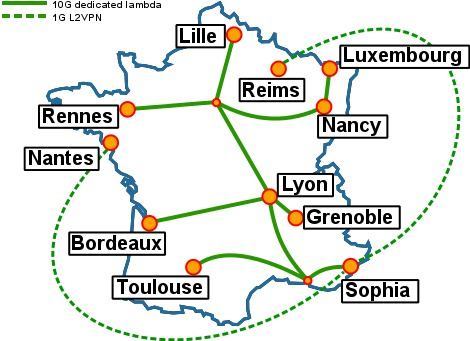
\includegraphics[scale=0.5]{images_custom/Renater5-g5k.jpg}
  \end{center}

\end{frame}


\begin{frame}[fragile]
    \frametitle{Presentation}
Technical features:
    \begin{itemize}
		\item reserve subnets and vlan (\textbf{kavlan})
		\item reserve storage capacity (iscsi / nfs)
		\item reconfigure the nodes for your experiment (\textbf{kadeploy})
	\end{itemize}

\end{frame}


\frame{
    \frametitle{Request your account and connect}
    \begin{enumerate}
      \item Fill the account request form on http://www.grid5000.fr

      \item Use the glocal access\\
        \begin{cmdline}
            \cmdlinenode{ssh <login>@access.grid5000.fr}
            \cmdlinenode{ssh luxembourg}
        \end{cmdline}

      \item Use the local access for the University
        \begin{cmdline}
            \cmdlinenode{ssh <login>@grid5000.uni.lu}
        \end{cmdline}
	\end{enumerate}
}

\frame{

  \frametitle{Objectives of the PS}

  \begin{itemize}
    \item Connect to Grid'5000
    \item Discover the key features of Grid'5000
    \item Use VM5K in order to deploy virtual machines on the grid
  \end{itemize}

  \begin{exampleblock}{Read the full subject of this PS here}
      \begin{itemize}
        \item http://bit.ly/1LvixgO
      \end{itemize}
  \end{exampleblock}

}

% ===============================================
\section{VM5K}

\frame{
  \frametitle{Presentation of VM5K}
    \begin{itemize}
		\item manage the reservation, locally or globally
		\item install the hosts with kadeploy
		\item configure the virtualization stack
		\item configure the network
		\item deploy the virtual machines
	\end{itemize}

  \begin{exampleblock}{Official website:}
      \begin{itemize}
        \item http://vm5k.readthedocs.org/
      \end{itemize}
  \end{exampleblock}
}

\frame{
  \begin{center}
      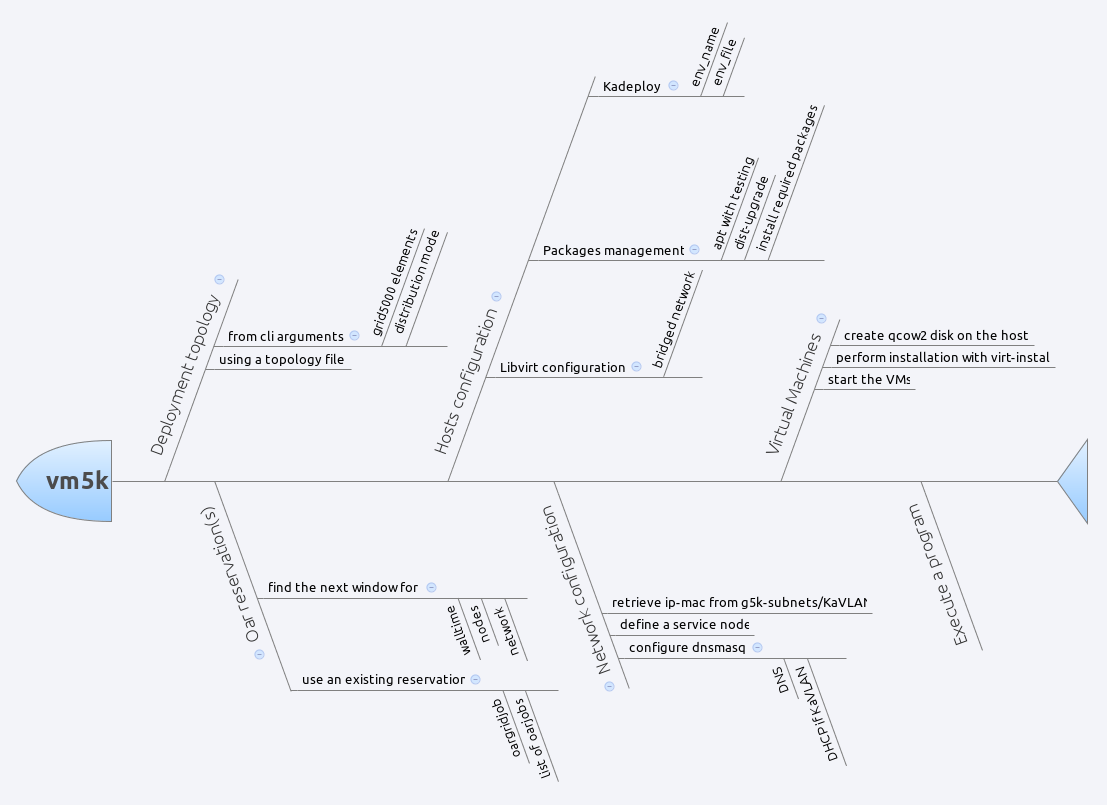
\includegraphics[scale=0.25]{images_custom/Vm5k_workflow}
  \end{center}
}

\frame{  
  \begin{center}
      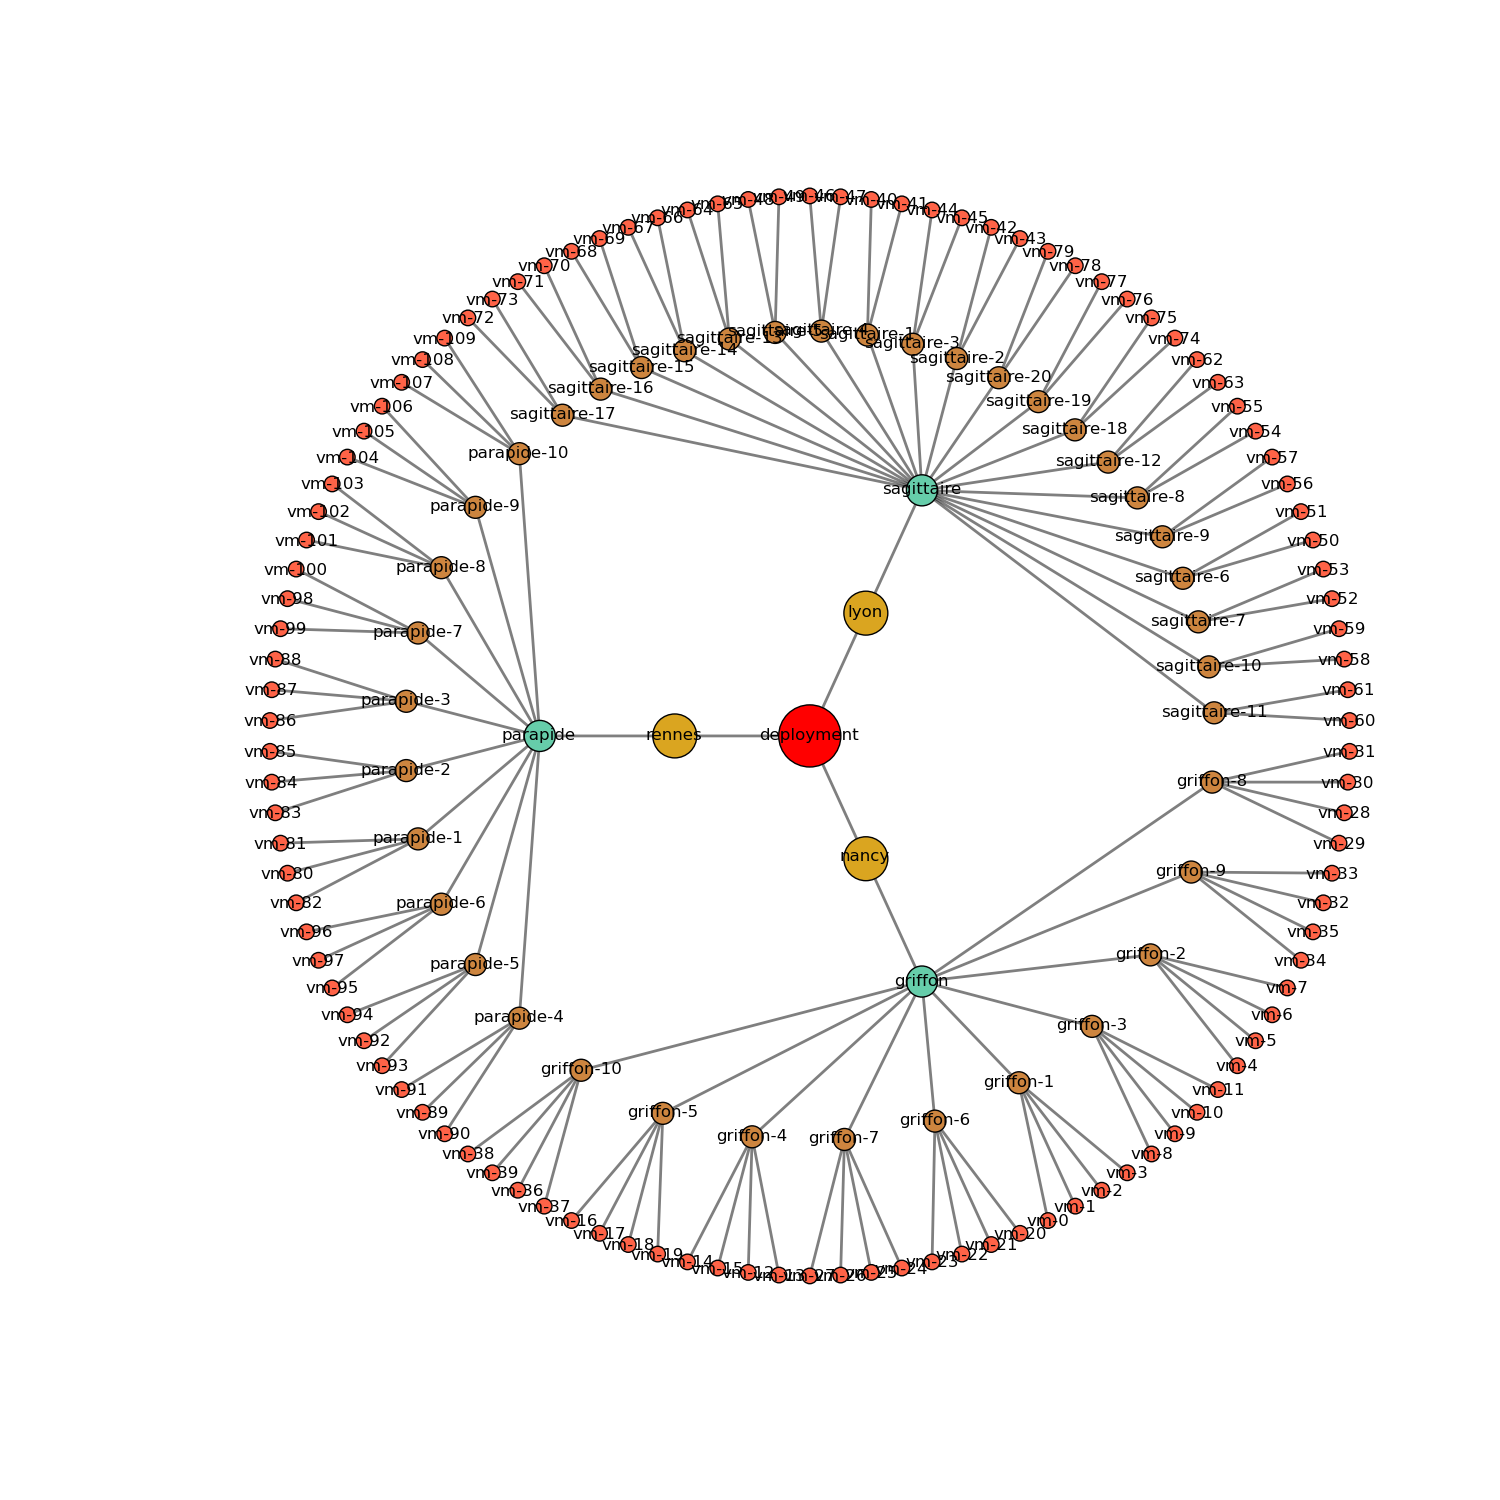
\includegraphics[scale=0.25]{images_custom/Vm5k_topology}
  \end{center}
}

\frame{
  \frametitle{Tutorial}
    \begin{itemize}
		\item VM5K tutorial
		
		\begin{itemize}
           \item http://ulhpc-tutorials.readthedocs.org/latest/advanced/vm5k/README/
        \end{itemize}
        
   		\item G5K Getting started tutorial
   		
   		\begin{itemize}
           \item https://www.grid5000.fr/mediawiki/index.php/Getting\_Started
        \end{itemize}
	\end{itemize}

}

\section*{Thank you for your attention...}
\frame{
  \frametitle{Questions?}
  \begin{center}
      
\includegraphics[scale=0.2]{question.jpg}
  \end{center}

  {\tiny
    \tableofcontents

  }
}

\end{document}

% ~~~~~~~~~~~~~~~~~~~~~~~~~~~~~~~~~~~~~~~~~~~~~~~~~~~~~~~~~~~~~~~~
% eof
%
% Local Variables:
% mode: latex
% mode: flyspell
% mode: auto-fill
% fill-column: 80
% End:
